\section{{Evidence for correlated trading} }


	In the previous sections, we have provided evidence consistent with the hypothesis that the presence of firms in the business groups can raise firms' co-movement. Although we don't have definitive insight into the specific channel that business groups can promote commonality, our analysis provides a useful overview.
	We claim that this relationship exists because the business group is an important proxy for the likelihood that trading in these stocks will be correlated. To better understand how the business group can generate co-movement in firms' returns, we now refine our basic analysis to consider other proxy measures for business group trading.
	We employ two proxies for business group trading that are designed to capture different trading motivations: turnover and institutional imbalance. While the first could be due to buying or selling of business groups, the latter reflects buying.
%	We employ one proxy for business group trading that is designed to capture  trading motivations: turnover which could be due to buying or selling of business groups.

		\captionsetup[subtable]{labelformat=parens}
			\renewcommand{\thesubtable}{\Alph{subtable}}

\subsection{{Turnover}}


	First, we should show that stocks in groups have a similar daily trading behavior. Accordingly, We use the turnover measure as a daily trading measures. For each firm we run time-series regressions of the firm's daily change in turnover, $ \Delta \text{TurnOver}_{i,t} $, on changes in market turnover,$ \Delta\text{TurnOver}_{Market,t}   $ , changes in the industry and business group portfolio's turnover,$ \Delta\text{TurnOver}_{Ind,t} $ and  $\Delta \text{TurnOver}_{Group,t} $ and  ,as well as control variables.
	We compute the daily change of turnover by this definition $ \Delta \text{TurnOver}_{i,t} = \ln(\frac{\text{TurnOver}_{i,t}}{\text{TurnOver}_{i,t-1}}) $. 
	We estimate the following regression for each stock across trading days in a given year separately, and cross-sectional averages of the estimated coefficients are reported, with t-statistics in parentheses :
	
		\begin{equation*}
	\begin{split}
		\Delta \text{Turnover}_{i,t} =  & \text{	}\alpha + \beta_{Market,t} \Delta \text{Turnover}_{Market,t}  
		+ \beta_{Ind,t} \Delta \text{Turnover}_{Ind,t} \\ & + \beta_{Group,t} \Delta \text{Turnover}_{Group,t} + \delta\text{Controls} + \varepsilon_{i,t}
	\end{split}
\end{equation*}
	  We control for lead and lag changes in the two portfolios and the firm's measures and size. We estimate that model with \cite{FamaMacBeth} method and adjust its standard errors with \cite{newey1987hypothesis} for seven periods.  As shown in Table \ref{turnover}, firms' change in turnover comes from market reaction and group's change (This result is robust to the different methods of weighting for portfolios). This observation shows that firms in one group trade together each day. 
	
	We use our previous methodology to investigate these results. We calculate correlation of $ \Delta \text{TurnOver} $ for founded pairs and examine its relation with our variables. Table \ref{mresult2-turnover} reports the estimation result, which confirms that pairs in the business groups lead to correlated trade. In addition, we study effect of  correlation of $ \Delta \text{TurnOver} $ on co-movement for founded pairs in table \ref{turncomovement}. These results suggest that business groups yield to future co-movement through correlated trading in that month.
  
  
  
  
  
  
{\begin{table}[htbp]
	\centering
	\caption{$\Delta \text{TurnOver}$ of firm and Business group\\
	This table reports \cite{FamaMacBeth} estimates of daily change in turnover ($ \Delta \text{TurnOver}_{i,t} = \ln(\frac{\text{TurnOver}_{i,t}}{\text{TurnOver}_{i,t-1}}) $) for all the firms in the market. The independent variables are change in turnover for Market, Insudtry, and Business group for that day. We exclude firm's change from associated groups to prevent spurious correlations. We calculate \cite{newey1987hypothesis} standard errors (seveb lags) of the \cite{FamaMacBeth} estimates that take into account autocorrelation in the cross-sectional slopes. We report the associated t-statistics in parentheses. }
		\label{turnover}
	\resizebox{!}{!}{
		{
\def\sym#1{\ifmmode^{#1}\else\(^{#1}\)\fi}
\begin{tabular}{l*{4}{c}}
\hline\hline
                    &\multicolumn{4}{c}{Dependent Variable: $\Delta \text{TurnOver}\_{i} $ }                 \\\cmidrule(lr){2-5}
                    &\multicolumn{1}{c}{(1)}         &\multicolumn{1}{c}{(2)}         &\multicolumn{1}{c}{(3)}         &\multicolumn{1}{c}{(4)}         \\
\hline
 $ \Delta \text{TurnOver}_{\text{Market}} $ &       0.416\sym{***}&       0.326\sym{***}&       0.252\sym{***}&       0.228\sym{***}\\
                    &     (12.25)         &      (5.35)         &      (6.41)         &      (4.24)         \\
[1em]
 $ \Delta \text{TurnOver}_{\text{Industry-i}} $ &       0.142\sym{***}&       0.213\sym{***}&      0.0335         &       0.167\sym{**} \\
                    &      (3.79)         &      (6.29)         &      (1.34)         &      (2.87)         \\
[1em]
 $ \Delta \text{TurnOver}_{\text{Group,-i}} $ &                     &                     &       0.330\sym{***}&       0.218\sym{***}\\
                    &                     &                     &     (12.74)         &      (3.80)         \\
\hline
Control             &          No         &         Yes         &          No         &         Yes         \\
Observations        &      854662         &      851772         &      333789         &      331263         \\
$ R^2 $             &       0.285         &       0.543         &       0.433         &       0.712         \\
\hline\hline
\multicolumn{5}{l}{\footnotesize \textit{t} statistics in parentheses}\\
\multicolumn{5}{l}{\footnotesize \sym{*} \(p<0.05\), \sym{**} \(p<0.01\), \sym{***} \(p<0.001\)}\\
\end{tabular}
}

	} 
\end{table}}

%\newgeometry{top=5mm, bottom=20mm}
	\begin{table}[htbp]
		\centering
		\caption{Simultaneous trade and Co-movement\\
		This table reports \cite{FamaMacBeth} estimates of the pairwise correlation in liquidity for the sample of stocks defined in Table \ref{t2-2}. The independent variables are updated monthly include our measure of institutional connectedness, the number of equal percents held block-holder, $\text{MFCAP}^*_{ij,t}$, and a series of controls at time t. We measure the negative of the absolute value of the difference in size and book-to-market ratio (BE/ME) percentile ranking across the two stocks in the pair (SameSize, and SameBM, respectively). All independent variables, excluding dummy variables, are rank-transformed and normalized to have a unit standard deviation. We calculate \cite{newey1987hypothesis} standard errors (four lags) of the \cite{FamaMacBeth} estimates that take into account autocorrelation in the cross-sectional slopes. We report the associated t-statistics in parentheses. Controls not shown here are reported in the Internet Appendix. We report estimates of regressions using variables to investigate the effect of common ownership and business group in Panel \subref{mresult2-turnover}. Panel \subref{turncomovement} shows the estimation result for investigating the effect of commonality in liquidity and co-movement. }
		
\subcaption{Correlation of $ \Delta \text{TurnOver} $ and interested variables}
		\label{mresult2-turnover}
		
		\resizebox{\textwidth}{!}{
			\centering
			{
\def\sym#1{\ifmmode^{#1}\else\(^{#1}\)\fi}
\begin{tabular}{l*{7}{c}}
\hline\hline
                    &\multicolumn{7}{c}{Dependent Variable:  Monthly Correlation of Delta turnover}                                                                           \\\cmidrule(lr){2-8}
                    &\multicolumn{1}{c}{(1)}         &\multicolumn{1}{c}{(2)}         &\multicolumn{1}{c}{(3)}         &\multicolumn{1}{c}{(4)}         &\multicolumn{1}{c}{(5)}         &\multicolumn{1}{c}{(6)}         &\multicolumn{1}{c}{(7)}         \\
\hline
SameGroup           &      0.0180\sym{***}&                     &      0.0173\sym{***}&                     &                     &      0.0150\sym{***}&      0.0168\sym{***}\\
                    &      (6.19)         &                     &      (5.53)         &                     &                     &      (4.89)         &      (5.40)         \\
[1em]
$ \text{MFCAP*} $   &                     &     0.00219\sym{**} &    0.000543         &     0.00115         &    0.000372         &    0.000363         &   -0.000413         \\
                    &                     &      (2.84)         &      (0.69)         &      (0.57)         &      (0.41)         &      (0.40)         &     (-0.37)         \\
[1em]
 $ (\text{MFCAP}^*) \times {\text{SameGroup} }  $ &                     &                     &                     &                     &                     &     0.00260         &     0.00296         \\
                    &                     &                     &                     &                     &                     &      (1.03)         &      (1.19)         \\
\hline
Sub-sample          &         All         &         All         &         All         &   SameGroup         &      Others         &         All         &         All         \\
Business Group FE   &          No         &          No         &          No         &          No         &          No         &          No         &         Yes         \\
Observations        &      294864         &      294864         &      294864         &       37076         &      257788         &      294864         &      294864         \\
\hline\hline
\multicolumn{8}{l}{\footnotesize \textit{t} statistics in parentheses}\\
\multicolumn{8}{l}{\footnotesize \sym{*} \(p<0.05\), \sym{**} \(p<0.01\), \sym{***} \(p<0.001\)}\\
\end{tabular}
}

		}
		\bigskip
		\subcaption{Correlation of $ \Delta \text{TurnOver} $ and Co-movement }
		\label{turncomovement}
		\resizebox{\textwidth}{!}{
			\centering
			{
\def\sym#1{\ifmmode^{#1}\else\(^{#1}\)\fi}
\begin{tabular}{l*{5}{c}}
\hline\hline
                    &\multicolumn{5}{c}{Dependent Variable:  Future Pairs's Comovement}                                           \\\cmidrule(lr){2-6}
                    &\multicolumn{1}{c}{(1)}         &\multicolumn{1}{c}{(2)}         &\multicolumn{1}{c}{(3)}         &\multicolumn{1}{c}{(4)}         &\multicolumn{1}{c}{(5)}         \\
\hline
 $ {\rho(\Delta \text{TurnOver})_{t+1}} $ &      0.0856\sym{***}&      0.0742\sym{***}&       0.152\sym{***}&      0.0611\sym{***}&      0.0743\sym{***}\\
                    &     (14.09)         &     (13.91)         &     (15.57)         &     (11.82)         &     (13.94)         \\
[1em]
 $ {\rho_t} $       &      0.0456\sym{***}&      0.0373\sym{***}&      0.0944\sym{***}&      0.0262\sym{***}&      0.0356\sym{***}\\
                    &     (11.44)         &     (10.58)         &     (13.66)         &      (6.57)         &     (10.71)         \\
\hline
Control             &          No         &         Yes         &         Yes         &         Yes         &         Yes         \\
Sub-sample          &       Total         &       Total         &   SameGroup         &      Others         &       Total         \\
Business Group FE   &          No         &          No         &          No         &          No         &         Yes         \\
Observations        &      338895         &      338895         &       41955         &      296940         &      338895         \\
\hline\hline
\multicolumn{6}{l}{\footnotesize \textit{t} statistics in parentheses}\\
\multicolumn{6}{l}{\footnotesize \sym{*} \(p<0.05\), \sym{**} \(p<0.01\), \sym{***} \(p<0.001\)}\\
\end{tabular}
}

		}
	
	\end{table}
\restoregeometry


Furthermore, we have to directly show that firms with a higher level of group turnover have a higher level of co-movement. So, we extract the annual average level of firms and monthly turnover for each month. We assume that the residual of the model belongs to the business groups. We expect firms in the groups to have a lower dispersion in their residuals than firms out of the groups. We calculate firms' residuals by the mentioned hypothesis. Its summary stats is in table \ref{tab:ResidualTrunSummary}. As we expected, residuals in business groups have a lower dispersion than others.


We calculate the standard error of firms' monthly turnover residuals in each business group. Groups' standard errors description is shown in table \ref{tab:ResidualTrunStdSummary} and time series in in figure \ref{fig:GroupedResSTD}. On average, the affiliated firms' standard error is lower than unaffiliated ones. For finding the relation between the standard error of monthly turnover residuals, we define a dummy variable for groups in the low level of standard error, which is lower than the median. For analysis, we restrict our investigations to a subsample of \textit{Same Group} and others and estimate our desired variable.   For further study, we use the interaction of \textit{Same Group} with our dummy variable for the full sample, which confirmed our prior results. As shown in table \ref{Turnovercrosssection}, pairs in the business groups of low dispersion have a higher level of co-movement than other firms.



{			\begin{table}[htbp]
\caption{Summary statistics}
	\centering
	\subcaption{Frims' Monthly residuals}
	\label{tab:ResidualTrunSummary}
	\resizebox{0.8\textwidth}{!}{
		\begin{tabular}{lrrrrrrrr}
\toprule
{} &  Firm\$\textbackslash times\$ Month &   mean &    std &    min &    25\% &    50\% &    75\% &    max \\
Grouped   &                     &        &        &        &        &        &        &        \\
\midrule
Ungrouped &                8050 & -0.001 &  0.822 & -4.789 & -0.509 & -0.016 &  0.504 &  4.407 \\
Grouped   &               18199 &  0.001 &  0.777 & -4.832 & -0.481 & -0.033 &  0.469 &  4.955 \\
\bottomrule
\end{tabular}

	}
	\bigskip
			\centering
			\subcaption{Groups' Monthly residuals' standard erros}
			\label{tab:ResidualTrunStdSummary}
			\resizebox{0.8\textwidth}{!}{
				\begin{tabular}{lrrrrrrrr}
\toprule
{} &  Group \$\textbackslash times\$ Month &   mean &    std &    min &    25\% &    50\% &    75\% &    max \\
Grouped   &                       &        &        &        &        &        &        &        \\
\midrule
Ungrouped &                    72 &  0.776 &  0.108 &  0.516 &  0.694 &  0.774 &  0.840 &  1.140 \\
Grouped   &                  2393 &  0.604 &  0.300 &  0.001 &  0.413 &  0.580 &  0.763 &  2.797 \\
\bottomrule
\end{tabular}

			}
		\end{table}
		
		
		
\begin{figure}[htbp]
	\centering
	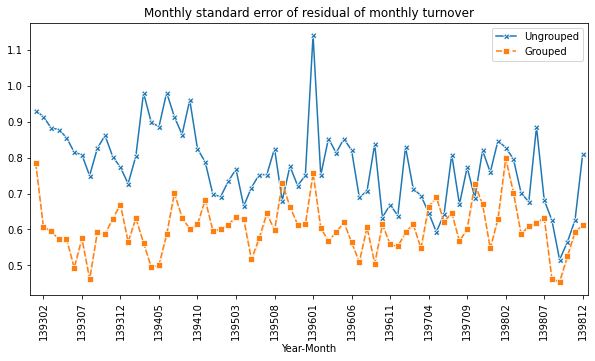
\includegraphics[width=0.85\linewidth]{Output/GroupedResSTD.eps}

	\caption{Time series of standard errors in residuals of Turnover for groups}
	\label{fig:GroupedResSTD}
\end{figure}


		\begin{table}[htbp]
			\centering
			\caption{Turnover and Imblance and Co-mivement\\
			This table reports \cite{FamaMacBeth} estimates of monthly cross-sectional regressions forecasting the correlation of daily \cite{fama1993differences}–\cite{Carhart4Factor} plus industry residuals in month t + 1 for the sample of stocks defined in Table \ref{t2-2}. The independent variables are updated monthly include our measure of institutional connectedness, the number of equal percents held block-holder, $\text{MFCAP}^*_{ij,t}$, and a series of controls at time t.
				We also define two dummy variables for the presence of the firm in the particular group. LowTurnoverStd is a dummy variable for groups in which the standard error of $\Delta \text{TurnOver}$ is lower than the median of each period and LowImbalanceStd for a group with low dispersion in institutional imbalances ($ \text{InsImb} = \frac{\text{Buy}_{\text{value}} - \text{Sell}_{\text{value}}}{\text{Buy}_{\text{value}} + \text{Sell}_{\text{value}}} $).  We measure the negative of the absolute value of the difference in size and book-to-market ratio (BE/ME) percentile ranking across the two stocks in the pair (SameSize, and SameBM, respectively). All independent variables, excluding dummy variables, are rank-transformed and normalized to have a unit standard deviation. We calculate \cite{newey1987hypothesis} standard errors (four lags) of the \cite{FamaMacBeth} estimates that take into account autocorrelation in the cross-sectional slopes. We report the associated t-statistics in parentheses. Controls not shown here are reported in the Internet Appendix. We report estimates of regressions using variables to investigate the effect of Turnover and Imbalance in Panel A and Panel B.}
				\subcaption{Low Turnover residual std groups and Co-movement}
				\label{Turnovercrosssection}	
			\resizebox{\textwidth}{!}{
				\centering
				{
\def\sym#1{\ifmmode^{#1}\else\(^{#1}\)\fi}
\begin{tabular}{l*{6}{c}}
\hline\hline
                &\multicolumn{6}{c}{Dependent Variable:  Future Pairs's co-movement}                                              \\\cmidrule(lr){2-7}
                &\multicolumn{1}{c}{(1)}         &\multicolumn{1}{c}{(2)}         &\multicolumn{1}{c}{(3)}         &\multicolumn{1}{c}{(4)}         &\multicolumn{1}{c}{(5)}         &\multicolumn{1}{c}{(6)}         \\
\hline
SameGroup       &   0.0208\sym{***}&   0.0210\sym{***}&                  &                  &   0.0137\sym{***}&   0.0113\sym{**} \\
                &   (7.91)         &   (7.77)         &                  &                  &   (3.73)         &   (3.19)         \\
[1em]
LowTurnoverStd  &                  & 0.000929         &   0.0171\sym{***}&-0.000982         & -0.00107         &  0.00279         \\
                &                  &   (0.84)         &   (3.88)         &  (-0.93)         &  (-1.04)         &   (1.39)         \\
[1em]
$ {\text{LowTurnoverStd} } \times {\text{SameGroup} }  $ &                  &                  &                  &                  &   0.0181\sym{***}&   0.0183\sym{***}\\
                &                  &                  &                  &                  &   (3.65)         &   (3.91)         \\
\hline
Sub-sample      &    Total         &    Total         &SameGroup         &   Others         &    Total         &    Total         \\
Business Group FE&       No         &       No         &       No         &       No         &       No         &      Yes         \\
Observations    &   354209         &   354209         &    43274         &   310935         &   354209         &   354209         \\
\hline\hline  \end{tabular}}

			}			
			\subcaption{Low Imbalance std groups and Co-movement}
			\label{Imbalance}
			\resizebox{\textwidth}{!}{
				{
\def\sym#1{\ifmmode^{#1}\else\(^{#1}\)\fi}
\begin{tabular}{l*{6}{c}}
\hline\hline
                    &\multicolumn{6}{c}{Dependent Variable:  Future Pairs's Comovement}                                                                 \\\cmidrule(lr){2-7}
                    &\multicolumn{1}{c}{(1)}         &\multicolumn{1}{c}{(2)}         &\multicolumn{1}{c}{(3)}         &\multicolumn{1}{c}{(4)}         &\multicolumn{1}{c}{(5)}         &\multicolumn{1}{c}{(6)}         \\
\hline
SameGroup           &      0.0208\sym{***}&      0.0206\sym{***}&                     &                     &     0.00619         &     0.00630\sym{*}  \\
                    &      (7.91)         &      (7.94)         &                     &                     &      (1.95)         &      (2.04)         \\
[1em]
LowImbalanceStd     &                     &    -0.00144         &      0.0282\sym{***}&    -0.00724\sym{***}&    -0.00610\sym{***}&    -0.00267         \\
                    &                     &     (-1.15)         &      (6.06)         &     (-5.74)         &     (-4.87)         &     (-1.85)         \\
[1em]
 $ \text{LowImbalanceStd} \times {\text{SameGroup} } $ &                     &                     &                     &                     &      0.0358\sym{***}&      0.0325\sym{***}\\
                    &                     &                     &                     &                     &      (8.57)         &      (7.48)         \\
\hline
Sub-sample          &       Total         &       Total         &   SameGroup         &      Others         &       Total         &       Total         \\
Business Group FE   &          No         &          No         &          No         &          No         &          No         &         Yes         \\
Observations        &      354209         &      354209         &       43274         &      310935         &      354209         &      354209         \\
\hline\hline
\multicolumn{7}{l}{\footnotesize \textit{t} statistics in parentheses}\\
\multicolumn{7}{l}{\footnotesize \sym{*} \(p<0.05\), \sym{**} \(p<0.01\), \sym{***} \(p<0.001\)}\\
\end{tabular}
}

			}
			
			
		\end{table}}




\FloatBarrier

%
%
\subsection{{Institutional Imbalance}}

	We should show that stocks in groups that trade together are traded in the same direction. So, for each firm, we calculate daily institutional imbalances, which is the net buying value of institutional investors relative to total traded value on that day ($ \text{InsImb} = \frac{\text{Buy}_{\text{value}} - \text{Sell}_{\text{value}}}{\text{Buy}_{\text{value}} + \text{Sell}_{\text{value}}} $ [\cite{seasholes2007predictable}]).
		We expect that institutional imbalances have a lower variation in groups due to the correlated tradings that the ultimate owner ordered to do. So, we calculate monthly institutional imbalances for firms at the first step. As we expected, firms in the business groups have a lower level of standard error in  imbalances (Table\ref{tab:ImbalanceInsMeanSummary}). Then, we calculate the monthly standard deviation of the group's imbalances and compare them to unaffiliated ones. The standard error is  $12.2\%$ and significantly (with a p-value of 0) lower than ungrouped firms. 
		
	{\begin{table}[htbp]
	\caption{Summary statistics}
		\centering
		\subcaption{Panel A: Frims' Monthly Imbalances}
			\label{tab:ImbalanceInsMeanSummary}%
		\resizebox{0.75\textwidth}{!}{
			\begin{tabular}{lrrrrrrrr}
\toprule
{} &  Group $\times$ Month &   mean &    std &  min &    25\% &    50\% &    75\% &  max \\
Grouped   &                       &        &        &      &        &        &        &      \\
\midrule
Ungrouped &                 20197 &  0.010 &  0.630 & -1.0 & -0.474 &  0.016 &  0.479 &  1.0 \\
Grouped   &                 12021 & -0.041 &  0.581 & -1.0 & -0.462 & -0.009 &  0.341 &  1.0 \\
\bottomrule
\end{tabular}

		}
	

		\subcaption{Panel B: Groups' Monthly Imbalances' standard erros}
				\label{tab:ImbalanceInsStdSummary}%
		\resizebox{0.75\textwidth}{!}{
			\begin{tabular}{lcccccccc}
\toprule
{} &  Group $\times$ Month &   mean &    std &   min &    25\% &    50\% &    75\% &    max \\
Grouped   &                       &        &        &       &        &        &        &        \\
\midrule
Ungrouped &                    72 &  0.624 &  0.054 &  0.48 &  0.601 &  0.631 &  0.655 &  0.735 \\
Grouped   &                  2057 &  0.503 &  0.251 &  0.00 &  0.337 &  0.503 &  0.647 &  1.414 \\
\bottomrule
\end{tabular}

		}
\end{table}}
	\begin{figure}[htbp]
		\centering
		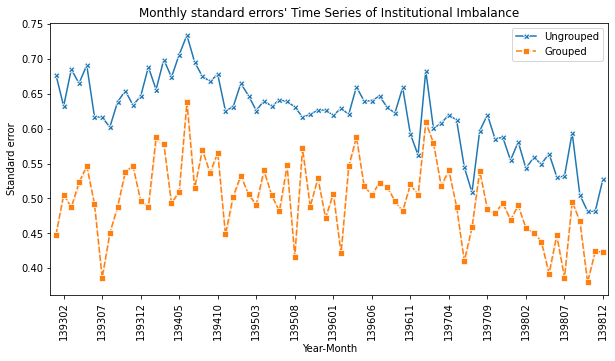
\includegraphics[width=0.85\linewidth]{Output/GroupedInsSTD.eps}
				\caption{Time series of standard errors in Imbalance for groups}
		\label{fig:GroupedInsSTD}
	\end{figure}
	
	According to the main hypothesis, we need to compare pairs in groups with low standard error and other pairs. For this purpose, we define \textbf{Low Imbalance std} dummy for groups whose average standard errors are lower than half of the sample. So, this dummy is equal to one if at least one pair's firms belong to the low imbalance std business group. We expect pairs in the same business groups with a low standard imbalance error to comove more than others. Table \ref{Imbalance} reports estimation results and confirms that pairs in the low imbalance std comove greater than others. 
	
%		{\begin{table}[htbp]
%			\centering
%			\caption{Estimation results for the relation between low imbalance std groups and co-movement}
%			\label{Imbalance}
%			\subcaption{\hl{heading}}
%			\resizebox{\textwidth}{!}{
%				{
\def\sym#1{\ifmmode^{#1}\else\(^{#1}\)\fi}
\begin{tabular}{l*{6}{c}}
\hline\hline
                    &\multicolumn{6}{c}{Dependent Variable:  Future Pairs's Comovement}                                                                 \\\cmidrule(lr){2-7}
                    &\multicolumn{1}{c}{(1)}         &\multicolumn{1}{c}{(2)}         &\multicolumn{1}{c}{(3)}         &\multicolumn{1}{c}{(4)}         &\multicolumn{1}{c}{(5)}         &\multicolumn{1}{c}{(6)}         \\
\hline
SameGroup           &      0.0208\sym{***}&      0.0206\sym{***}&                     &                     &     0.00619         &     0.00630\sym{*}  \\
                    &      (7.91)         &      (7.94)         &                     &                     &      (1.95)         &      (2.04)         \\
[1em]
LowImbalanceStd     &                     &    -0.00144         &      0.0282\sym{***}&    -0.00724\sym{***}&    -0.00610\sym{***}&    -0.00267         \\
                    &                     &     (-1.15)         &      (6.06)         &     (-5.74)         &     (-4.87)         &     (-1.85)         \\
[1em]
 $ \text{LowImbalanceStd} \times {\text{SameGroup} } $ &                     &                     &                     &                     &      0.0358\sym{***}&      0.0325\sym{***}\\
                    &                     &                     &                     &                     &      (8.57)         &      (7.48)         \\
\hline
Sub-sample          &       Total         &       Total         &   SameGroup         &      Others         &       Total         &       Total         \\
Business Group FE   &          No         &          No         &          No         &          No         &          No         &         Yes         \\
Observations        &      354209         &      354209         &       43274         &      310935         &      354209         &      354209         \\
\hline\hline
\multicolumn{7}{l}{\footnotesize \textit{t} statistics in parentheses}\\
\multicolumn{7}{l}{\footnotesize \sym{*} \(p<0.05\), \sym{**} \(p<0.01\), \sym{***} \(p<0.001\)}\\
\end{tabular}
}

%			}
%	\end{table}}



\FloatBarrier

